In the second to last iteration we discovered that our simulator didn't degrade anything (Figure~\ref{fig:wrong}), this was discovered so late because non of the tests targeted degradation, we only tested if the reaction speed changed. Either the solver library (SBMLsimulator) was wrong or the SBML format used was. After some testing and help from Alexey, the problem found was indeed the SBML format.\\

\begin{figure}[h!]
	\centering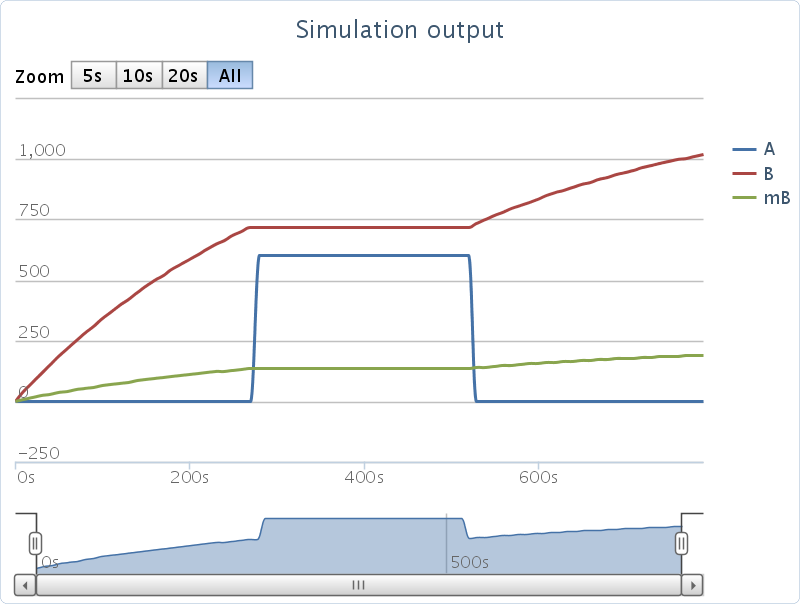
\includegraphics[scale=0.35]{../../screenshots/2012-05-31-not-output.png}
	\caption{Wrong output, B doesn't degrade.}
	\label{fig:wrong}
\end{figure}

\noindent The SBML format that is used for the simulation requires a list of species and a list of reactions. These reactions each have a set of reactants, products and modifiers:
\begin{itemize}
	\item reactants are the fuel of the reactions, the reactants decrease as the reaction occurs,
	\item products are what the reaction produces in the end, the products increase as the reaction occurs,
	\item modifiers can speed up or slow down the reaction, but their concentration doesn't change in the reaction.
\end{itemize}
In our simulation we have two reactions: transcription and translation. The transcription reaction produces mRNA (that encodes for a specific protein) from a gene sequence with help from transcription factors. The translation reaction produces the protein from the mRNA. On top of this degradation takes place: the proteins and mRNA degrade over time.\\
\\
In our SBML file the degradation didn't have a separate reaction, which caused a problem given that the degradation reaction required a different set of reactants, products and modifiers from the transcription and translation reactions.\\
The transcription reaction produces something from a gene sequence. The degradation reactions need to degrade to something, but it's not producing something from a gene sequence, so putting the degradation in the same reaction as the transcription (or translation) reaction would be wrong since they have different reactants and different products.\\

\begin{wrapfigure}{l}{8cm}
	\centering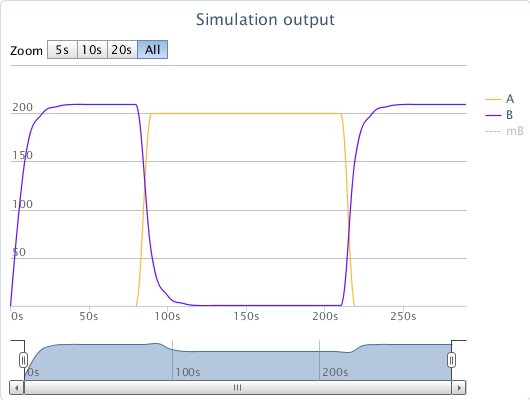
\includegraphics[scale=0.5]{../../screenshots/2012-06-14-not-output.png}
	\caption{Correct output, B degrades.}
	\label{fig:correct}
\end{wrapfigure}

To fix this (Figure~\ref{fig:correct}) we split the transcription and translation reactions such that the degradations got their own reactions, this allowed us to specify different reactants, products and modifiers for the degradation.
